% =====================================================================
%  Exponentials & Logarithms -- Worked Example Set, Chapter 3G--3L
%  Year 10 Mathematical Methods (10 Methods Primer), 2026
%
%  Every section runs: Key ideas -> I do -> We do -> Fix it -> You do.
%  All examples are original; none are copied from the textbook.
%
%  TWO BUILDS FROM THIS ONE SOURCE
%    Ch3G-L_Example_Set.tex          student copy -- every blank empty
%    Ch3G-L_Example_Set_Teacher.tex  teacher copy -- defines \teacheranswers
%                                    (every \defans) and then \input's this
%                                    file, so blanks and answers print in red.
%  The teacher wrapper and its PDF are gitignored: answer keys never ship
%  as a plain file (ROADMAP.md, "Staff material"). Keep this file free of
%  answers -- they live only in the wrapper, keyed by the names used in
%  \blank, \cell and \tans below. A key missing from the wrapper prints as
%  ??key?? in the teacher copy, so grep the teacher PDF for "??".
%
%  Build each with xelatex three times (contents page refs, then LastPage).
% =====================================================================
\documentclass[11pt]{article}
\usepackage[a4paper,margin=20mm,headsep=6mm]{geometry}
\usepackage{amsmath,amssymb}
% lmodern where it is installed (as for the other primer booklets);
% the OpenType Latin Modern otherwise, so the booklet still builds.
\IfFileExists{lmodern.sty}{\usepackage[T1]{fontenc}\usepackage{lmodern}}{%
  \usepackage{fontspec}\setmainfont{Latin Modern Roman}\setsansfont{Latin Modern Sans}}
\usepackage{xcolor}
\usepackage{tikz}
\usetikzlibrary{arrows.meta}
\usepackage[most]{tcolorbox}
\usepackage{enumitem}
\usepackage{fancyhdr}
\usepackage{needspace}
\usepackage{lastpage}
\usepackage{array}
\usepackage{environ}

% ---------- Palette (matches the Ch5/7 and Ch6 question booklets) ----------
\definecolor{chalk}{HTML}{2F6F8F}
\definecolor{chalkdk}{HTML}{24576F}
\definecolor{amber}{HTML}{D98A3D}
\definecolor{ink}{HTML}{1A2B34}
\definecolor{inksoft}{HTML}{4A5F68}
\definecolor{paper}{HTML}{F6F4EF}
\definecolor{line}{HTML}{DFE3E0}
% gradual-release colours, as on the site (tokens.css --ido/--wedo/--youdo)
\definecolor{ido}{HTML}{33508F}
\definecolor{wedo}{HTML}{A8610F}
\definecolor{youdo}{HTML}{1E7D56}
\definecolor{fixit}{HTML}{C23B32}
% red: worked first rows (scaffolds) and the teacher copy's answers
\definecolor{scaf}{HTML}{C62828}
\color{ink}
\setlength{\parindent}{0pt}\setlength{\parskip}{3pt}
\AtBeginDocument{\setlength{\abovedisplayskip}{6pt}\setlength{\belowdisplayskip}{6pt}%
  \setlength{\abovedisplayshortskip}{4pt}\setlength{\belowdisplayshortskip}{6pt}}

% ---------- Student / teacher switch ----------
\newif\ifteacher
\makeatletter
\newcommand{\defans}[2]{\@namedef{kans@#1}{#2}}
\newcommand{\getans}[1]{\@ifundefined{kans@#1}{\textbf{??#1??}}{\@nameuse{kans@#1}}}
\makeatother
\ifdefined\teacheranswers \teachertrue \teacheranswers \fi
% \blank{width}{key} -- a write-in blank; filled in red in the teacher copy.
% Answers are \smash'ed and \tans takes no height, so the teacher copy
% paginates exactly like the student copy and page numbers agree.
\newcommand{\blank}[2]{\ifteacher\underline{\makebox[#1]{\smash{\color{scaf}\getans{#2}}}}\else\underline{\makebox[#1]{}}\fi}
% \cell{key} -- a write-in table cell
\newcommand{\cell}[1]{\ifteacher{\color{scaf}\getans{#1}}\fi}
% \tans{key} -- the teacher copy's answer, written on the ruled lines that follow
\newcommand{\tans}[1]{\ifteacher\par\nointerlineskip
  \vbox to 0pt{\hsize=\linewidth\color{scaf}\setlength{\baselineskip}{\rulepitch}\setlength{\lineskiplimit}{-\maxdimen}%
    \setlength{\parskip}{0pt}\vskip -1pt\hbox{}\noindent\textsf{\bfseries Answer.}\ \getans{#1}\par\vss}\fi}
% \scaf{...} -- a worked first row, shown to students in red
\newcommand{\scaf}[1]{{\color{scaf}#1}}

% ---------- Running heads ----------
\pagestyle{fancy}\fancyhf{}
\renewcommand{\headrulewidth}{0.4pt}
\renewcommand{\headrule}{\hbox to\headwidth{\color{line}\leaders\hrule height 0.4pt\hfill}}
\lhead{\small\color{inksoft}\textsc{Exponentials \& Logarithms : 3G--3L}}
\rhead{\small\color{inksoft}Year 10 Methods : \ifteacher Example Set : \textcolor{scaf}{\bfseries Teacher copy}\else Worked Example Set\fi}
\cfoot{\small\color{inksoft}Page \thepage\ of \pageref{LastPage}}

% ---------- Section furniture ----------
\newcommand{\sectionband}[3]{\needspace{5\baselineskip}\vspace{2pt}
  \begin{tcolorbox}[enhanced,colback=chalk,colframe=chalk,boxrule=0pt,left=12pt,right=12pt,top=8pt,bottom=8pt,arc=4pt,
      overlay={\node[anchor=east,text=white,opacity=0.9] at ([xshift=-12pt]frame.east) {\small\textsf{#3}};}]
    {\color{white}\large\bfseries\textsf{#1}\quad #2}\end{tcolorbox}}
\newcounter{example}
\newcounter{qnum}
\newcommand{\cursec}{}
% Every section starts on a new page.
\newcommand{\startsection}[3]{\clearpage\renewcommand{\cursec}{#1}\setcounter{qnum}{0}%
  \sectionband{#1}{#2}{#3}\label{sec:#1}}

\newtcolorbox{refbox}{enhanced,breakable,colback=paper,colframe=line,boxrule=0.6pt,left=12pt,right=12pt,top=8pt,bottom=8pt,arc=3pt}
\newtcolorbox{idobox}{enhanced,colback=ido!4,colframe=ido!40,boxrule=0.7pt,left=12pt,right=12pt,top=8pt,bottom=8pt,arc=3pt,borderline west={3pt}{0pt}{ido}}
\newtcolorbox{wedobox}{enhanced,colback=wedo!4,colframe=wedo!40,boxrule=0.7pt,left=12pt,right=12pt,top=8pt,bottom=8pt,arc=3pt,borderline west={3pt}{0pt}{wedo}}
\newtcolorbox{fixbox}{enhanced,colback=fixit!3,colframe=fixit!40,boxrule=0.7pt,left=12pt,right=12pt,top=8pt,bottom=8pt,arc=3pt,borderline west={3pt}{0pt}{fixit}}
\newtcolorbox{studentwork}{enhanced,colback=white,colframe=fixit!45,boxrule=0.6pt,arc=2pt,left=10pt,right=10pt,top=5pt,bottom=5pt}

\newcommand{\phase}[2]{\tcbox[on line,colback=#1,colframe=#1,boxrule=0pt,arc=2pt,left=3pt,right=3pt,top=1.5pt,bottom=1.5pt]{\color{white}\scriptsize\sffamily\bfseries #2}}

% ---------- Filling the page instead of leaving gaps ----------
% Writing lines are 8 mm apart everywhere, so the teacher copy's answers
% (\tans) can be set on the same pitch and sit on the lines.
\newlength{\rulepitch}\setlength{\rulepitch}{8mm}
\newcommand{\ruledline}{\vbox to\rulepitch{\vfil\hbox to\linewidth{\color{line!140!white}\leaders\hrule height 0.3pt\hfill}}}
% Ruled lines from here to the foot of the page.
\newcommand{\linesfill}{\leaders\ruledline\vfill}
\newcommand{\filllines}{\par\vspace{2pt}\linesfill\null}
\newcommand{\notesfill}{\par\vspace{8pt}{\small\color{inksoft}\textsf{Notes}}\par\linesfill}
% \placeorfill{height}{filler}: if the next block needs more room than is
% left on the page, fill what is left with the filler and start a new page.
\makeatletter
\newcommand{\placeorfill}[2]{\par\penalty-100\begingroup
  \dimen@=#1\relax \dimen@ii=\pagegoal \advance\dimen@ii-\pagetotal
  \ifdim\dimen@>\dimen@ii \ifdim\dimen@ii>30pt #2\fi \newpage\fi
  \endgroup}
\makeatother
% Example boxes are set first, measured, then placed whole.
\newsavebox{\exbox}
\newcommand{\placeexample}{\placeorfill{\dimexpr\ht\exbox+\dp\exbox+10pt\relax}{\notesfill}%
  \vspace{6pt}\noindent\usebox{\exbox}\par}
% Worked example: heading on its own line, then the task below it.
\NewEnviron{idoex}[1]{\refstepcounter{example}%
  \sbox{\exbox}{\begin{minipage}{\linewidth}\begin{idobox}
  \phase{ido}{I DO}\ \ {\bfseries\color{ido}Example \theexample\ --- #1}\par\vspace{4pt}\BODY\end{idobox}\end{minipage}}%
  \placeexample}
\NewEnviron{wedoex}[1]{\refstepcounter{example}%
  \sbox{\exbox}{\begin{minipage}{\linewidth}\begin{wedobox}
  \phase{wedo}{WE DO}\ \ {\bfseries\color{wedo}Example \theexample\ --- #1}\par\vspace{4pt}\BODY\end{wedobox}\end{minipage}}%
  \placeexample}
\NewEnviron{fixit}{%
  \sbox{\exbox}{\begin{minipage}{\linewidth}\begin{fixbox}
  \phase{fixit}{FIX IT}\ \ {\bfseries\color{fixit}Spot the error}\par\vspace{4pt}\BODY\end{fixbox}\end{minipage}}%
  \placeexample}

\newcommand{\soln}{\par\vspace{3pt}{\bfseries\color{ido}Solution}}
\newcommand{\together}{\par\vspace{3pt}{\bfseries\color{wedo}Work through it together}\par}
\newcommand{\ianswer}[1]{\par\vspace{2pt}{\bfseries\color{ido}Answer.}\ #1\par}
\newcommand{\why}[1]{\text{\small\color{inksoft}#1}}
\newcommand{\tip}[2]{\par\vspace{5pt}{\small{\bfseries\color{chalkdk}#1}\ \color{inksoft}#2}\par}
\newenvironment{parts}{\begin{enumerate}[leftmargin=22pt,itemsep=4pt,topsep=3pt,label=\textbf{(\alph*)}]}{\end{enumerate}}
% Roomy line spacing for We do working, so blanks can be written in.
\newenvironment{scaffold}{\par\vspace{2pt}\begin{list}{}{\leftmargin=0pt\itemsep=11pt\topsep=4pt}}{\end{list}}

% Your turn
\newcommand{\yourturn}{\placeorfill{16\baselineskip}{\notesfill}\vspace{10pt}
  {\phase{youdo}{YOU DO}\ \ \bfseries\color{youdo}\large Your turn --- Section \cursec}\;\textcolor{inksoft}{\small(show all working)}\par\vspace{2pt}}
\newcommand{\yq}[1][9]{\refstepcounter{qnum}\placeorfill{#1\baselineskip}{\linesfill}\vspace{8pt}%
  {\bfseries\color{chalkdk}Question \cursec.\theqnum}\par\nopagebreak\vspace{1pt}}
% \yqs{key}: a question heading with a "Section: ___" blank at the right (mixed practice)
\newcommand{\yqs}[2][9]{\refstepcounter{qnum}\placeorfill{#1\baselineskip}{\linesfill}\vspace{8pt}%
  {\bfseries\color{chalkdk}Question \cursec.\theqnum}\hfill{\small Section:}\ \blank{16mm}{#2}\par\nopagebreak\vspace{1pt}}
\newcommand{\worklines}[1]{\par\vspace{2pt}\foreach \n in {1,...,#1}{\nointerlineskip\ruledline}\par\vspace{2pt}}

% Write-in tables: 1.5 cm rows, ruled on every side.
\newcolumntype{C}[1]{>{\centering\arraybackslash}m{#1}}
\newcolumntype{L}[1]{>{\raggedright\arraybackslash}m{#1}}
\newcommand{\wrow}{\rule[-0.72cm]{0pt}{1.5cm}}

% ---------- Figures ----------
\newcommand{\figGrowthDecay}{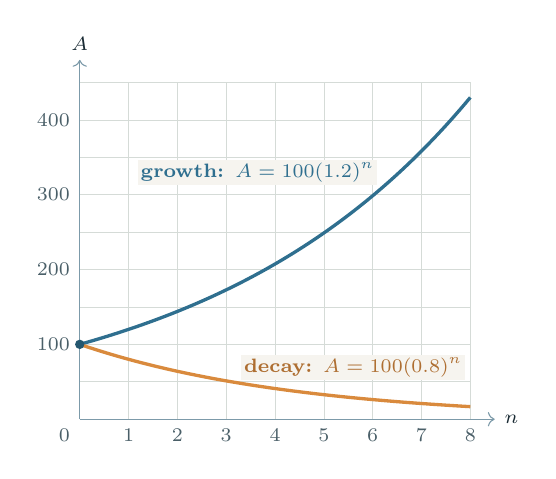
\begin{tikzpicture}[x=0.62cm,y=0.0095cm,font=\scriptsize]
  \draw[line!130!white,very thin] (0,0) grid[xstep=1,ystep=50] (8,450);
  \draw[chalkdk!60,->] (0,0)--(8.5,0) node[right,ink]{$n$};
  \draw[chalkdk!60,->] (0,0)--(0,480) node[above,ink]{$A$};
  \foreach \x in {1,...,8} \node[below,inksoft] at (\x,0) {\x};
  \foreach \y in {100,200,300,400} \node[left,inksoft] at (0,\y) {\y};
  \node[below left,inksoft] at (0,0) {0};
  \draw[chalk,very thick,domain=0:8,samples=60,smooth] plot (\x,{100*1.2^\x});
  \draw[amber,very thick,domain=0:8,samples=60,smooth] plot (\x,{100*0.8^\x});
  \fill[chalkdk] (0,100) circle (1.7pt);
  \node[chalk,fill=paper,inner sep=1pt,font=\scriptsize\bfseries,left] at (6.1,330) {growth: $A=100(1.2)^n$};
  \node[amber!80!black,fill=paper,inner sep=1pt,font=\scriptsize\bfseries,above] at (5.6,52) {decay: $A=100(0.8)^n$};
\end{tikzpicture}}

\newcommand{\figLogStrip}{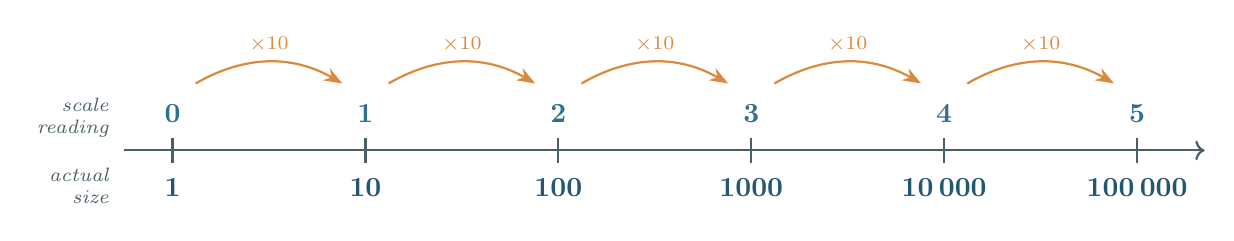
\begin{tikzpicture}[x=2.45cm,font=\small]
  \draw[inksoft,thick,->] (-0.25,0)--(5.35,0);
  \foreach \k/\v in {0/1,1/10,2/100,3/1000,4/10\,000,5/100\,000}{
    \draw[inksoft,thick] (\k,-0.16)--(\k,0.16);
    \node[above=2pt,chalk,font=\bfseries] at (\k,0.16) {\k};
    \node[below=2pt,chalkdk,font=\bfseries] at (\k,-0.16) {\v};}
  \foreach \k in {0,...,4} \draw[amber,thick,-{Stealth}] (\k+0.12,0.85) to[bend left=30] node[above,font=\scriptsize\bfseries]{$\times 10$} (\k+0.88,0.85);
  \node[left,inksoft,font=\scriptsize\itshape,align=right] at (-0.28,0.42) {scale\\reading};
  \node[left,inksoft,font=\scriptsize\itshape,align=right] at (-0.28,-0.45) {actual\\size};
\end{tikzpicture}}

% one step of a log axis, 1000 to 10 000; the teacher copy shows the marks
\newcommand{\figLogAxis}{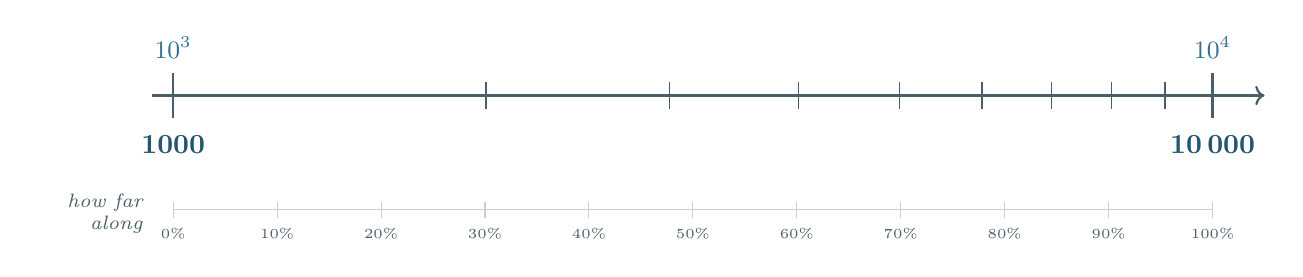
\begin{tikzpicture}[x=13.2cm,font=\small]
  \draw[inksoft,thick,->] (-0.02,0)--(1.05,0);
  \draw[inksoft,thick] (0,-0.28)--(0,0.28) (1,-0.28)--(1,0.28);
  \foreach \v in {2000,3000,...,9000}{\pgfmathsetmacro\p{log10(\v)-3}\draw[inksoft] (\p,-0.17)--(\p,0.17);}
  \node[below=3pt,chalkdk,font=\bfseries] at (0,-0.28) {1000};
  \node[below=3pt,chalkdk,font=\bfseries] at (1,-0.28) {10\,000};
  \node[above=2pt,chalk] at (0,0.28) {$10^{3}$};
  \node[above=2pt,chalk] at (1,0.28) {$10^{4}$};
  \draw[line!170!white] (0,-1.45)--(1,-1.45);
  \foreach \q in {0,10,...,100}{\draw[line!170!white] (\q/100,-1.55)--(\q/100,-1.35);
     \node[font=\tiny,inksoft] at (\q/100,-1.75) {\q\%};}
  \node[left,font=\scriptsize\itshape,inksoft,align=right] at (-0.02,-1.5) {how far\\along};
  \path[use as bounding box] (-0.14,-1.95) rectangle (1.06,0.82);
  \ifteacher
    \foreach \v in {2000,3000,...,9000}{\pgfmathsetmacro\p{log10(\v)-3}\node[scaf,font=\tiny,below=1pt] at (\p,-0.17) {\v};}
    \fill[scaf] (0.699,0) circle (3pt);
    \draw[scaf,thick] (0.699,0.12)--(0.699,0.3) node[above,font=\small\bfseries]{5000};
    \draw[scaf,thick,dashed] (0.5,0.12)--(0.5,0.3) node[above,font=\small\bfseries]{halfway $\approx 3162$};
  \fi
\end{tikzpicture}}

\newcommand{\figThreeX}{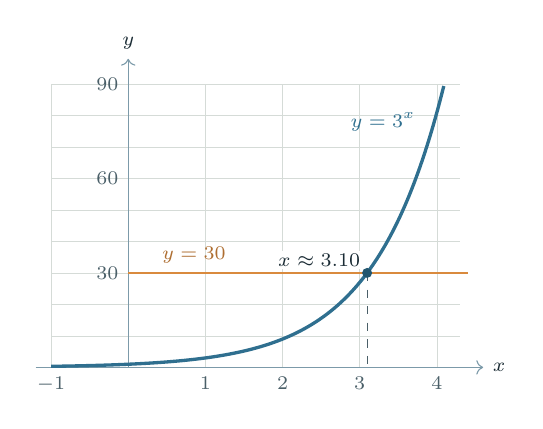
\begin{tikzpicture}[x=0.98cm,y=0.04cm,font=\scriptsize]
  \draw[line!130!white,very thin] (-1,0) grid[xstep=1,ystep=10] (4.3,90);
  \draw[chalkdk!60,->] (-1.2,0)--(4.6,0) node[right,ink]{$x$};
  \draw[chalkdk!60,->] (0,0)--(0,98) node[above,ink]{$y$};
  \foreach \x in {-1,1,2,3,4} \node[below,inksoft] at (\x,0) {$\x$};
  \foreach \y in {30,60,90} \node[left,inksoft] at (0,\y) {\y};
  \draw[amber,thick] (0,30)--(4.4,30);
  \node[amber!80!black,font=\scriptsize\bfseries,above] at (0.85,30) {$y=30$};
  \draw[chalk,very thick,domain=-1:4.09,samples=80,smooth] plot (\x,{3^\x});
  \draw[inksoft,dashed] (3.096,30)--(3.096,0);
  \fill[chalkdk] (3.096,30) circle (1.8pt);
  \node[ink,fill=white,inner sep=1pt,above left] at (3.05,31) {$x\approx 3.10$};
  \node[chalk,font=\scriptsize\bfseries,left] at (3.85,78) {$y=3^x$};
\end{tikzpicture}}

\begin{document}

% =====================================================================
%  COVER
% =====================================================================
\thispagestyle{empty}
\begin{tikzpicture}[remember picture,overlay]
  \fill[chalk](current page.north west)rectangle([yshift=-64mm]current page.north east);
  \node[anchor=north west,text=white,align=left]at([xshift=20mm,yshift=-19mm]current page.north west)
    {{\Huge\bfseries\textsf{Exponentials \& Logarithms}}\\[3mm]{\LARGE\textsf{Worked Example Set\ifteacher\ : Teacher Copy\fi}}\\[3mm]
     {\large\textsf{Chapter 3G--3L : Year 10 Mathematical Methods : 2026}}};
\end{tikzpicture}
\vspace{58mm}

{\large Name: \underline{\makebox[95mm]{}}\qquad Class: \underline{\makebox[30mm]{}}}

\vspace{6mm}
\begin{refbox}
{\bfseries\color{chalkdk}How to use this booklet}\par\vspace{3pt}
Every section from 3G to 3L runs in the same order.
\begin{itemize}[leftmargin=16pt,itemsep=5pt,topsep=5pt]
  \item[] \phase{chalk}{KEY IDEAS}\ \ The rule for the section, all in one place. Come back to it whenever you are stuck.
  \item[] \phase{ido}{I DO}\ \ Fully worked examples. Your teacher talks through each line. The grey notes on the right say \emph{why} each step happens.
  \item[] \phase{wedo}{WE DO}\ \ Examples we finish together. Fill in each blank as the class works it out.
  \item[] \phase{fixit}{FIX IT}\ \ A student's working with one mistake in it. Find the mistake, explain it, then fix it.
  \item[] \phase{youdo}{YOU DO}\ \ Questions to try on your own, with space to write.
\end{itemize}
\vspace{3pt}{\color{scaf}Red writing} in a table is a worked first row. It shows you what to do in the rows below.\par
\vspace{3pt}{\small\color{inksoft}Sections 3K and 3L are marked \textsf{10A}: they are extension. In every section, write the rule before you calculate, and answer in words when the question has a context.}
\end{refbox}

\vspace{4mm}
\begin{refbox}
{\bfseries\color{chalkdk}Contents}\par\vspace{4pt}
\renewcommand{\arraystretch}{1.35}
\begin{tabular*}{\linewidth}{@{}p{12mm}@{}l@{\extracolsep{\fill}}r@{}}
\textbf{3G} & Exponential growth and decay & \pageref{sec:3G} \\
\textbf{3H} & Compound interest & \pageref{sec:3H} \\
\textbf{3I} & Introducing logarithms & \pageref{sec:3I} \\
\textbf{3J} & Logarithmic scales & \pageref{sec:3J} \\
\textbf{3K} & Laws of logarithms \textcolor{inksoft}{\small(10A)} & \pageref{sec:3K} \\
\textbf{3L} & Solving exponential equations using logarithms \textcolor{inksoft}{\small(10A)} & \pageref{sec:3L} \\
\textbf{Mix} & Mixed practice --- which section? & \pageref{sec:Mixed} \\
\end{tabular*}
\end{refbox}

\vfill
{\small\color{inksoft}Sections follow \emph{Essential Mathematics for the Victorian Curriculum 10 \& 10A}, 3rd ed., Chapter 3. Every example and question in this booklet is original material written for this course.}

% =====================================================================
%  3G
% =====================================================================
\startsection{3G}{Exponential growth and decay}{CORE}

\begin{refbox}
{\bfseries\color{chalkdk}Key ideas}\par\vspace{4pt}
\begin{minipage}[t]{0.53\linewidth}
\textbf{Growth:}\quad $A = A_0\left(1 + \dfrac{r}{100}\right)^{n}$\\[5pt]
\textbf{Decay:}\quad\ $A = A_0\left(1 - \dfrac{r}{100}\right)^{n}$\\[5pt]
$A_0$ is the starting amount, $r$ is the percentage change each time period, and $n$ is the number of time periods.\\[6pt]
\renewcommand{\arraystretch}{1.3}
\begin{tabular}{|l|c|}\hline
\textbf{The question says \ldots} & \textbf{Multiply by} \\\hline
grows by 20\% each hour & $1.2$ \\\hline
increases by 3.5\% each year & $1.035$ \\\hline
loses 15\% each year & $0.85$ \\\hline
decreases by 2\% each month & $0.98$ \\\hline
\end{tabular}\\[6pt]
Multiplier more than 1: \textbf{growth}.\\
Multiplier between 0 and 1: \textbf{decay}.
\end{minipage}\hfill
\begin{minipage}[t]{0.44\linewidth}\vspace{0pt}\centering\figGrowthDecay\\[2pt]
{\scriptsize\color{inksoft}Both start at 100. Growth multiplies by 1.2 each period; decay multiplies by 0.8.}
\end{minipage}
\end{refbox}

\begin{idoex}{A growing colony}
A colony of 500 bacteria increases by 20\% every hour. Write a rule for the number of bacteria, $N$, after $n$ hours. Then find the number of bacteria after 6 hours.
\soln
\begin{align*}
\text{multiplier} &= 1 + \tfrac{20}{100} = 1.2 && \why{increases, so add the rate to 1}\\
N &= 500(1.2)^{n} && \why{the rule}\\
N &= 500(1.2)^{6} && \why{substitute $n = 6$}\\
  &= 500 \times 2.985984 = 1492.992 && \why{calculate}\\
  &\approx 1493 && \why{a whole number of bacteria}
\end{align*}
\ianswer{After 6 hours there are about 1493 bacteria.}
\tip{Why not $500 + 6 \times 100$?}{The 20\% is taken of the \emph{new} amount each hour, so each increase is bigger than the last: $500 \to 600 \to 720 \to 864 \to \cdots$, which is $+100$, $+120$, $+144$, \ldots\ Adding the same amount each time is linear. Multiplying by the same number each time is exponential.}
\end{idoex}

\begin{idoex}{Medicine leaving the body}
A patient takes a 40\,mg dose of a medicine. Each hour, the body removes 15\% of the medicine that is still present.
\begin{parts}
  \item Write a rule for the amount of medicine, $M$\,mg, after $t$ hours.
  \item Find the amount left after 4 hours, correct to one decimal place.
  \item After 4 hours, is more or less than half of the dose left?
\end{parts}
\soln
\begin{align*}
&\textbf{(a)} & \text{multiplier} &= 1 - \tfrac{15}{100} = 0.85 && \why{removes 15\%, so 85\% stays}\\
&& M &= 40(0.85)^{t} && \why{the rule}\\[3pt]
&\textbf{(b)} & M &= 40(0.85)^{4} = 40 \times 0.52200625 && \why{substitute $t = 4$}\\
&& &= 20.88\ldots \approx 20.9 && \why{one decimal place}\\[3pt]
&\textbf{(c)} & \tfrac{1}{2} \times 40 &= 20 \text{ and } 20.9 > 20 && \why{compare with half the dose}
\end{align*}
\ianswer{(a) $M = 40(0.85)^{t}$ \quad (b) about 20.9\,mg \quad (c) just \textbf{more} than half of the dose is left.}
\tip{The multiplier is what stays.}{Losing 15\% means keeping 85\%, so write $0.85$, never $0.15$.}
\end{idoex}

\begin{wedoex}{What does the rule tell us?}
For each rule, write the starting amount, whether it shows growth or decay, and the percentage rate for each time period. The first row is done for you.
\par\vspace{6pt}
\begin{center}\renewcommand{\arraystretch}{1}
\begin{tabular}{|C{33mm}|C{24mm}|C{40mm}|C{44mm}|}\hline
\textbf{Rule} & \textbf{Starting amount} & \textbf{Growth or decay?} & \textbf{Rate each period} \\\hline
\wrow $V = 12\,000(0.92)^{t}$ & \scaf{$12\,000$} & \scaf{decay, because $0.92 < 1$} & \scaf{$1 - 0.92 = 0.08$, so 8\%} \\\hline
\wrow $P = 350(1.045)^{n}$ & \cell{3G-w3-b1} & \cell{3G-w3-b2} & \cell{3G-w3-b3} \\\hline
\wrow $A = 60(2)^{n}$ & \cell{3G-w3-c1} & \cell{3G-w3-c2} & \cell{3G-w3-c3} \\\hline
\wrow $M = 2.4(0.7)^{t}$ & \cell{3G-w3-d1} & \cell{3G-w3-d2} & \cell{3G-w3-d3} \\\hline
\end{tabular}\end{center}
\vspace{4pt}
{\bfseries\color{wedo}Say it}, for the rule for $M$:\par\vspace{8pt}
``The rule starts at \blank{18mm}{3G-w3-say1} and \blank{18mm}{3G-w3-say2} by \blank{14mm}{3G-w3-say3}\% each \blank{18mm}{3G-w3-say4}.''
\end{wedoex}

\begin{wedoex}{When does the town drop below 6000?}
A town of 8000 people is shrinking by 5\% each year. After how many whole years will the population first be below 6000?
\together
\begin{scaffold}
\item \textbf{Step 1.}\ The multiplier is \blank{22mm}{3G-w4-mult}, so the rule is $P = $ \blank{40mm}{3G-w4-rule}.
\item \textbf{Step 2.}\ Try values of $n$. The first row is done for you.
\end{scaffold}
\begin{center}\renewcommand{\arraystretch}{1}
\begin{tabular}{|C{20mm}|C{56mm}|C{36mm}|C{28mm}|}\hline
\textbf{Years, $n$} & \textbf{Working} & \textbf{Population $P$} \newline {\small(nearest whole)} & \textbf{Below 6000?} \\\hline
\wrow \scaf{3} & \scaf{$8000(0.95)^{3} = 6859$} & \scaf{6859} & \scaf{No} \\\hline
\wrow 4 & \cell{3G-w4-r4w} & \cell{3G-w4-r4p} & \cell{3G-w4-r4y} \\\hline
\wrow 5 & \cell{3G-w4-r5w} & \cell{3G-w4-r5p} & \cell{3G-w4-r5y} \\\hline
\wrow 6 & \cell{3G-w4-r6w} & \cell{3G-w4-r6p} & \cell{3G-w4-r6y} \\\hline
\end{tabular}\end{center}
\begin{scaffold}
\item \textbf{Step 3.}\ The population first drops below 6000 after \blank{16mm}{3G-w4-ans} years.
\end{scaffold}
{\small\color{inksoft}Looking ahead: in Section 3L you will solve $0.95^{n} = 0.75$ exactly with logarithms, and get $n \approx 5.61$.}
\end{wedoex}

\begin{fixit}
A car worth \$20\,000 loses 15\% of its value each year. Find its value after 1 year.
\begin{studentwork}
{\small\bfseries\color{fixit}A student wrote:}\par\vspace{4pt}
$V = 20\,000(0.15)^{n}$, so after 1 year $V = 20\,000 \times 0.15 = \$3000$.
\end{studentwork}
Explain the mistake. Then write the correct working.
\tans{3G-fix}
\worklines{4}
\end{fixit}

\yourturn

\yq A painting bought for \$1200 increases in value by 4\% each year.
\begin{parts}
  \item Write a rule for its value, $V$ dollars, after $n$ years.
  \item Find its value after 5 years, correct to the nearest cent.
\end{parts}
\tans{3G-y1}
\worklines{3}

\yq A machine bought for \$65\,000 loses 10\% of its value each year. Find its value after 4 years.
\tans{3G-y2}
\worklines{3}

\yq[8] Write the multiplier for each change.
\begin{parts}
  \item grows by 2.5\% each year \hfill \blank{30mm}{3G-y3a}
  \item loses 2.5\% each year \hfill \blank{30mm}{3G-y3b}
  \item doubles every hour \hfill \blank{30mm}{3G-y3c}
\end{parts}

\yq[8] The rule $A = 750(0.94)^{t}$ gives an amount after $t$ years.
\begin{parts}
  \item What is the starting amount? \hfill \blank{40mm}{3G-y4a}
  \item Is this growth or decay? \hfill \blank{40mm}{3G-y4b}
  \item What is the percentage rate each year? \hfill \blank{40mm}{3G-y4c}
\end{parts}

\yq An investment of \$2000 grows by 8\% each year. Try values of $n$ to find after how many whole years it is first worth more than \$3000.
\tans{3G-y5}
\filllines

% =====================================================================
%  3H
% =====================================================================
\startsection{3H}{Compound interest}{CORE}

\begin{refbox}
{\bfseries\color{chalkdk}Key ideas}\par\vspace{4pt}
\begin{minipage}[t]{0.50\linewidth}
\textbf{Compound interest}\\[4pt]
$A = P\left(1 + \dfrac{r}{100}\right)^{n}$\qquad interest $I = A - P$\\[5pt]
$P$ is the principal (the starting money), $r$ is the rate \textbf{per period}, and $n$ is the number of \textbf{periods}.
\end{minipage}\hfill
\begin{minipage}[t]{0.45\linewidth}
\textbf{Simple interest}, for comparison\\[4pt]
$I = \dfrac{P \times r \times t}{100}$\\[5pt]
The same interest every year. Round money to the nearest cent, at the \textbf{end} only.
\end{minipage}\par\vspace{8pt}
\begin{center}\renewcommand{\arraystretch}{1.35}
\begin{tabular}{|l|c|c|}\hline
\textbf{Compounded} & \textbf{Rate per period} & \textbf{Number of periods in $t$ years} \\\hline
annually & $r$ & $t$ \\\hline
half-yearly & $r \div 2$ & $2t$ \\\hline
quarterly & $r \div 4$ & $4t$ \\\hline
monthly & $r \div 12$ & $12t$ \\\hline
\end{tabular}\end{center}
{\small Divide the rate by the number of periods in a year. Multiply the years by the same number.}
\end{refbox}

\begin{idoex}{Compounded annually}
\$6000 is invested at 5\% p.a., compounded annually, for 4 years.
\begin{parts}
  \item Find the final amount.
  \item Find the interest earned.
\end{parts}
\soln
\begin{align*}
&& P &= 6000,\quad r = 5,\quad n = 4 && \why{write $P$, $r$, $n$ first}\\
&\textbf{(a)} & A &= 6000\left(1 + \tfrac{5}{100}\right)^{4} = 6000(1.05)^{4} && \why{substitute}\\
&& &= 6000 \times 1.21550625 = 7293.0375 && \why{calculate}\\
&& &\approx 7293.04 && \why{nearest cent}\\[3pt]
&\textbf{(b)} & I &= 7293.04 - 6000 = 1293.04 && \why{interest $= A - P$}
\end{align*}
\ianswer{(a) The final amount is \$7293.04. \quad (b) The interest earned is \$1293.04.}
\tip{Keep the full calculator value.}{Rounding $1.05^{4}$ to $1.22$ first gives $6000 \times 1.22 = \$7320$, which is \$26.96 too much.}
\end{idoex}

\begin{idoex}{Compounded monthly}
\$10\,000 is invested at 6\% p.a., compounded monthly, for 3 years. Find the final amount.
\soln
\begin{align*}
r &= 6 \div 12 = 0.5 && \why{rate per month}\\
n &= 3 \times 12 = 36 && \why{number of months}\\
A &= 10\,000\left(1 + \tfrac{0.5}{100}\right)^{36} = 10\,000(1.005)^{36} && \why{substitute}\\
  &\approx 11\,966.81 && \why{nearest cent}
\end{align*}
\ianswer{After 3 years the investment is worth \$11\,966.81.}
\tip{Compare with compounding annually.}{$10\,000(1.06)^{3} = \$11\,910.16$. Compounding monthly earns \$56.65 more, because the interest starts earning interest sooner.}
\end{idoex}

\begin{wedoex}{How much more does compounding earn?}
\$4000 is invested for 5 years at 7\% p.a. How much more does compound interest (compounded annually) earn than simple interest?
\together
\begin{scaffold}
\item \textbf{Simple interest.}\ \ $I = \dfrac{4000 \times 7 \times 5}{100} = $ \blank{24mm}{3H-w7-si}, so the final amount is \blank{24mm}{3H-w7-sa}.
\item \textbf{Compound interest.}\ \ $A = 4000\,\Big($\blank{16mm}{3H-w7-mult}$\Big)^{5} = $ \blank{28mm}{3H-w7-ca}
\item \textbf{Difference.}\ \ \blank{22mm}{3H-w7-d1} $-$ \blank{22mm}{3H-w7-d2} $=$ \blank{22mm}{3H-w7-d3}
\item \textbf{Answer.}\ \ Compound interest earns \$\blank{22mm}{3H-w7-ans} more.
\item \textbf{Think.}\ \ Simple interest pays \$280 every year. Why does compound interest pay more than \$280 in each year after the first?\\[6pt]
\blank{\linewidth}{3H-w7-think}
\end{scaffold}
\end{wedoex}

\begin{wedoex}{Which account pays more?}
Mai has \$8000 to invest for 3 years.\par
Account A pays 6\% p.a., compounded annually.\par
Account B pays 5.9\% p.a., compounded monthly.\par
Which account gives more money, and how much more?
\together
\begin{scaffold}
\item \textbf{Predict first.}\ \ Circle one:\quad Account A \qquad Account B
\item \textbf{Account A.}\ \ Multiplier \blank{16mm}{3H-w8-am}, \quad $n = $ \blank{12mm}{3H-w8-an}, \quad so $A = \$$\blank{26mm}{3H-w8-aa}
\item \textbf{Account B.}\ \ Rate per month $= \dfrac{5.9}{12}\%$, \quad number of months $n = $ \blank{14mm}{3H-w8-bn}
\item[] \hspace{19mm}$A = 8000\left(1 + \dfrac{5.9}{1200}\right)^{36} = \$$\blank{26mm}{3H-w8-ba}
\item \textbf{Answer.}\ \ Account \blank{10mm}{3H-w8-win} gives \$\blank{20mm}{3H-w8-diff} more.
\end{scaffold}
{\small\color{inksoft}Notice: the account with the \emph{lower} rate can still win, because it compounds 12 times a year.}
\end{wedoex}

\begin{fixit}
\$10\,000 is invested at 6\% p.a., compounded monthly, for 3 years. Find the final amount.
\begin{studentwork}
{\small\bfseries\color{fixit}A student wrote:}\par\vspace{4pt}
The monthly rate is 0.5\%, so $A = 10\,000(1.005)^{3} = \$10\,150.75$.
\end{studentwork}
Explain the mistake. Then write the correct working.
\tans{3H-fix}
\worklines{4}
\end{fixit}

\yourturn

\yq \$2500 is invested at 3\% p.a., compounded annually, for 6 years. Find the interest earned.
\tans{3H-y1}
\worklines{3}

\yq \$15\,000 is invested at 4.8\% p.a., compounded monthly, for 2 years. Find the final amount.
\tans{3H-y2}
\worklines{3}

\yq \$7000 is invested at 8\% p.a., compounded quarterly, for 3 years. Find the final amount.
\tans{3H-y3}
\worklines{3}

\yq \$900 is invested at 5.2\% p.a., compounded half-yearly, for $t$ years. Write a rule for the final amount, $A$. You do not need to calculate it.
\tans{3H-y4}
\worklines{2}

\yq \$12\,000 is borrowed at 9\% p.a., compounded annually. No repayments are made.
\begin{parts}
  \item How much is owed after 3 years?
  \item How much of this is interest?
\end{parts}
\tans{3H-y5}
\filllines

% =====================================================================
%  3I
% =====================================================================
\startsection{3I}{Introducing logarithms}{CORE}

\begin{refbox}
{\bfseries\color{chalkdk}Key ideas}\par\vspace{4pt}
\begin{minipage}[t]{0.52\linewidth}
$\log_{a} x = y \quad\text{means}\quad a^{y} = x$\\[5pt]
A logarithm asks: ``$a$ to \textbf{what power} gives $x$?''\\
The log \textbf{is} the power.
\end{minipage}\hfill
\begin{minipage}[t]{0.44\linewidth}
\textbf{Two anchors:}\ $\log_{a} 1 = 0$, because $a^{0} = 1$\\
\phantom{\textbf{Two anchors:}}\ $\log_{a} a = 1$, because $a^{1} = a$\\[4pt]
\textbf{Calculator:} the \textsf{log} button is base 10, so $\log 1000$ means $\log_{10} 1000 = 3$.
\end{minipage}\par\vspace{8pt}
\begin{center}\renewcommand{\arraystretch}{1.35}
\begin{tabular}{|c|c|l|}\hline
\textbf{Index form} & \textbf{Log form} & \textbf{Say it} \\\hline
$2^{3} = 8$ & $\log_{2} 8 = 3$ & ``2 to the power 3 gives 8'' \\\hline
$10^{2} = 100$ & $\log_{10} 100 = 2$ & ``10 to the power 2 gives 100'' \\\hline
\end{tabular}\end{center}
\end{refbox}

\begin{idoex}{Swap between the two forms}
\begin{parts}
  \item Write in log form:\quad $2^{5} = 32$, \quad $10^{-3} = 0.001$, \quad $9^{\frac{1}{2}} = 3$
  \item Write in index form:\quad $\log_{3} 81 = 4$, \quad $\log_{5} 0.04 = -2$, \quad $\log_{8} 2 = \tfrac{1}{3}$
\end{parts}
\soln\par
\begin{minipage}[t]{0.48\linewidth}
\textbf{(a)}
\begin{align*}
2^{5} = 32 &\;\Rightarrow\; \log_{2} 32 = 5\\
10^{-3} = 0.001 &\;\Rightarrow\; \log_{10} 0.001 = -3\\
9^{\frac{1}{2}} = 3 &\;\Rightarrow\; \log_{9} 3 = \tfrac{1}{2}
\end{align*}
\end{minipage}\hfill
\begin{minipage}[t]{0.48\linewidth}
\textbf{(b)}
\begin{align*}
\log_{3} 81 = 4 &\;\Rightarrow\; 3^{4} = 81\\
\log_{5} 0.04 = -2 &\;\Rightarrow\; 5^{-2} = 0.04\\
\log_{8} 2 = \tfrac{1}{3} &\;\Rightarrow\; 8^{\frac{1}{3}} = 2
\end{align*}
\end{minipage}
\tip{The move.}{The base stays the base. The power on one side is the answer on the other side.}
\end{idoex}

\begin{idoex}{Ask ``what power?''}
Evaluate without a calculator.
\begin{parts}
  \item $\log_{2} 64$
  \item $\log_{7} 1$
  \item $\log_{4} \dfrac{1}{16}$
  \item $\log_{27} 3$
\end{parts}
\soln
\begin{align*}
&\textbf{(a)} & 2^{6} &= 64, &&\text{so } \log_{2} 64 = 6 && \why{2 to what power gives 64?}\\
&\textbf{(b)} & 7^{0} &= 1, &&\text{so } \log_{7} 1 = 0 && \why{any base to the power 0 is 1}\\
&\textbf{(c)} & 4^{-2} &= \tfrac{1}{4^{2}} = \tfrac{1}{16}, &&\text{so } \log_{4} \tfrac{1}{16} = -2 && \why{a fraction needs a negative power}\\
&\textbf{(d)} & 27^{\frac{1}{3}} &= \sqrt[3]{27} = 3, &&\text{so } \log_{27} 3 = \tfrac{1}{3} && \why{smaller than the base: a root}
\end{align*}
\tip{Patterns to look for.}{The answer is a fraction like $\frac{1}{16}$: a \textbf{negative} power. The answer is smaller than the base, like 3 from 27: a \textbf{fraction} power. The answer is 1: the log is \textbf{0}, whatever the base.}
\end{idoex}

\begin{wedoex}{Rewrite in index form, then solve}
Find the value of $x$. Write each equation in index form first.
\together
\begin{scaffold}
\item \textbf{(a)}\ \ $\log_{2} x = 5$ \quad index form: \blank{32mm}{3I-w11-a1} \quad so $x = $ \blank{20mm}{3I-w11-a2}
\item \textbf{(b)}\ \ $\log_{x} 49 = 2$ \quad index form: \blank{32mm}{3I-w11-b1} \quad so $x = $ \blank{20mm}{3I-w11-b2}
\item \textbf{(c)}\ \ $\log_{10} x = -2$ \quad index form: \blank{32mm}{3I-w11-c1} \quad so $x = $ \blank{20mm}{3I-w11-c2}
\item \textbf{(d)}\ \ $\log_{3} 27 = x$ \quad index form: \blank{32mm}{3I-w11-d1} \quad so $x = $ \blank{20mm}{3I-w11-d2}
\end{scaffold}
{\small\color{inksoft}In (b), $x = -7$ also gives $x^{2} = 49$, but the base of a logarithm must be positive.}
\end{wedoex}

\begin{wedoex}{Between which two whole numbers?}
Without a calculator, find the two whole numbers that each logarithm lies between.
\together
\begin{scaffold}
\item \textbf{(a)}\ \ $\log_{2} 20$:\quad \blank{20mm}{3I-w12-a1} $< 20 <$ \blank{20mm}{3I-w12-a2}, \ so $\log_{2} 20$ is between \blank{10mm}{3I-w12-a3} and \blank{10mm}{3I-w12-a4}.
\item \textbf{(b)}\ \ $\log_{10} 350$:\quad \blank{20mm}{3I-w12-b1} $< 350 <$ \blank{20mm}{3I-w12-b2}, \ so $\log_{10} 350$ is between \blank{10mm}{3I-w12-b3} and \blank{10mm}{3I-w12-b4}.
\item[] \hspace{8mm}Check (b) on the calculator: $\log 350 = $ \blank{24mm}{3I-w12-b5}
\item \textbf{(c)}\ \ $\log_{3} 100$:\quad \blank{20mm}{3I-w12-c1} $< 100 <$ \blank{20mm}{3I-w12-c2}, \ so $\log_{3} 100$ is between \blank{10mm}{3I-w12-c3} and \blank{10mm}{3I-w12-c4}.
\end{scaffold}
{\small\color{inksoft}(a) and (c) are not base 10, so the \textsf{log} button cannot find them directly. Section 3L shows how --- and this estimate is how you will check that answer.}
\end{wedoex}

\begin{fixit}
Evaluate $\log_{2} 8$.
\begin{studentwork}
{\small\bfseries\color{fixit}A student wrote:}\par\vspace{4pt}
$\log_{2} 8 = 4$, because $8 \div 2 = 4$.
\end{studentwork}
Explain the mistake. Then write the correct working.
\tans{3I-fix}
\worklines{3}
\end{fixit}

\yourturn

\yq Write in log form.
\begin{parts}
  \item $6^{3} = 216$ \hfill \blank{45mm}{3I-y1a}
  \item $10^{4} = 10\,000$ \hfill \blank{45mm}{3I-y1b}
  \item $4^{-1} = 0.25$ \hfill \blank{45mm}{3I-y1c}
\end{parts}

\yq Write in index form.
\begin{parts}
  \item $\log_{2} 128 = 7$ \hfill \blank{45mm}{3I-y2a}
  \item $\log_{5} 1 = 0$ \hfill \blank{45mm}{3I-y2b}
  \item $\log_{16} 4 = \tfrac{1}{2}$ \hfill \blank{45mm}{3I-y2c}
\end{parts}

\yq[10] Evaluate without a calculator.
\begin{parts}
  \item $\log_{5} 125$ \hfill \blank{30mm}{3I-y3a}
  \item $\log_{10} 0.0001$ \hfill \blank{30mm}{3I-y3b}
  \item $\log_{9} 3$ \hfill \blank{30mm}{3I-y3c}
  \item $\log_{2} \dfrac{1}{8}$ \hfill \blank{30mm}{3I-y3d}
\end{parts}

\yq Solve for $x$.
\begin{parts}
  \item $\log_{x} 64 = 3$
  \item $\log_{4} x = 3$
\end{parts}
\tans{3I-y4}
\worklines{3}

\yq Between which two whole numbers does $\log_{2} 50$ lie? Explain how you know.
\tans{3I-y5}
\filllines

% =====================================================================
%  3J
% =====================================================================
\startsection{3J}{Logarithmic scales}{CORE}

\begin{refbox}
{\bfseries\color{chalkdk}Key ideas}\par\vspace{2pt}
\begin{center}\figLogStrip\end{center}
\vspace{2pt}
One step on a log scale is $\times 10$ in real life. Two readings $k$ apart: the actual sizes differ by a factor of $10^{k}$. \textbf{Subtract} the readings, then raise 10 to that power.
\begin{center}\renewcommand{\arraystretch}{1.35}
\begin{tabular}{|l|l|}\hline
\textbf{Scale} & \textbf{One step means} \\\hline
Richter magnitude & $\times 10$ amplitude of shaking \\\hline
pH (a \textbf{lower} pH is \textbf{more} acidic) & $\times 10$ acidity \\\hline
decibels (dB) & every \textbf{10\,dB} is $\times 10$ intensity \\\hline
\end{tabular}\end{center}
\end{refbox}

\begin{idoex}{Comparing earthquakes}
\begin{parts}
  \item How many times larger is the amplitude of a magnitude 7.3 earthquake than the amplitude of a magnitude 4.3 earthquake?
  \item How many times larger is the amplitude of a magnitude 6.5 earthquake than the amplitude of a magnitude 5.0 earthquake?
\end{parts}
\soln
\begin{align*}
&\textbf{(a)} & 7.3 - 4.3 &= 3 && \why{difference in readings}\\
&& 10^{3} &= 1000 && \why{each step is $\times 10$}\\[3pt]
&\textbf{(b)} & 6.5 - 5.0 &= 1.5 && \why{difference in readings}\\
&& 10^{1.5} &\approx 31.6 && \why{between $10^{1} = 10$ and $10^{2} = 100$, as expected}
\end{align*}
\ianswer{(a) 1000 times larger. \quad (b) About 32 times larger.}
\end{idoex}

\begin{idoex}{How much more intense is the sound?}
A lawnmower measures 90\,dB. Normal conversation measures 60\,dB. How many times more intense is the lawnmower's sound?
\soln
\begin{align*}
90 - 60 &= 30 \text{ dB} && \why{difference in readings}\\
30 \div 10 &= 3 \text{ steps} && \why{one step is 10 dB}\\
10^{3} &= 1000 && \why{each step is $\times 10$}
\end{align*}
\ianswer{The lawnmower's sound is 1000 times more intense.}
\tip{Decibels are different.}{On the Richter and pH scales one step is 1. On the decibel scale one step is 10\,dB, so the factor is $10^{\text{difference} \div 10}$. A 3\,dB difference is $10^{0.3} \approx 2$: about twice as intense.}
\end{idoex}

\begin{wedoex}{Which is more acidic, and how many times?}
Remember: a \textbf{lower} pH is \textbf{more} acidic.
\begin{parts}
  \item Vinegar has pH 3. Black coffee has pH 5.
  \item Normal rain has pH 5.6. Seawater has pH 8.1.
\end{parts}
\together
\begin{scaffold}
\item \textbf{(a)}\ \ More acidic: \blank{24mm}{3J-w15-a1} \qquad Steps apart, $k$: \blank{14mm}{3J-w15-a2} \qquad $10^{k} = $ \blank{20mm}{3J-w15-a4} times
\item \textbf{(b)}\ \ More acidic: \blank{24mm}{3J-w15-b1} \qquad Steps apart, $k$: \blank{14mm}{3J-w15-b2} \qquad $10^{k} \approx $ \blank{20mm}{3J-w15-b4} times
\end{scaffold}
\end{wedoex}

\begin{wedoex}{From ``times bigger'' back to a reading}
\begin{parts}
  \item An aftershock has $\dfrac{1}{100}$ of the amplitude of a magnitude 6.8 earthquake. What is the magnitude of the aftershock?
  \item An earthquake has 1000 times the amplitude of a magnitude 3.9 tremor. What is the magnitude of the earthquake?
\end{parts}
\together
\begin{scaffold}
\item \textbf{(a)}\ \ $\dfrac{1}{100} = 10^{k}$ with $k = $ \blank{12mm}{3J-w16-a1}, so the reading moves \blank{10mm}{3J-w16-a2} steps \blank{16mm}{3J-w16-a3} (up or down).\\[8pt]
Magnitude of the aftershock $=$ \blank{20mm}{3J-w16-a4}
\item \textbf{(b)}\ \ $1000 = 10^{k}$ with $k = $ \blank{12mm}{3J-w16-b1}, so the reading moves \blank{10mm}{3J-w16-b2} steps \blank{16mm}{3J-w16-b3} (up or down).\\[8pt]
Magnitude of the earthquake $=$ \blank{20mm}{3J-w16-b4}
\end{scaffold}
\end{wedoex}

\begin{wedoex}{Where does 5000 go on a log axis?}
The axis below is a log axis from 1000 to 10\,000. The eight small ticks are 2000, 3000, \ldots, 9000.
\begin{center}\figLogAxis\end{center}
\together
\begin{scaffold}
\item \textbf{(a)}\ \ $\log 1000 = 3$ and $\log 10\,000 = 4$. Use a calculator: $\log 5000 = $ \blank{24mm}{3J-w17-a}
\item \textbf{(b)}\ \ So 5000 sits \blank{14mm}{3J-w17-b}\% of the way from 1000 to 10\,000. Mark 5000 on the axis.
\item \textbf{(c)}\ \ The number exactly halfway along is $10^{3.5} = $ \blank{20mm}{3J-w17-c}. Mark it on the axis.
\item \textbf{(d)}\ \ Label the small ticks 2000 to 9000. What do you notice about how they are spaced?\\[6pt]
\blank{\linewidth}{3J-w17-d}
\end{scaffold}
\end{wedoex}

\begin{fixit}
Compare the amplitude of a magnitude 6 earthquake with the amplitude of a magnitude 3 earthquake.
\begin{studentwork}
{\small\bfseries\color{fixit}A student wrote:}\par\vspace{4pt}
The magnitude 6 earthquake is twice as big, because $6 = 2 \times 3$.
\end{studentwork}
Explain the mistake. Then write the correct working.
\tans{3J-fix}
\worklines{3}
\end{fixit}

\yourturn

\yq How many times larger is the amplitude of a magnitude 8.1 earthquake than the amplitude of a magnitude 5.1 earthquake?
\tans{3J-y1}
\worklines{3}

\yq How many times larger is the amplitude of a magnitude 5.7 earthquake than the amplitude of a magnitude 5.2 earthquake?
\tans{3J-y2}
\worklines{3}

\yq A rock concert measures 110\,dB. Busy traffic measures 80\,dB. How many times more intense is the sound of the rock concert?
\tans{3J-y3}
\worklines{3}

\yq Solution A has pH 4. Solution B has pH 7.
\begin{parts}
  \item Which solution is more acidic?
  \item How many times more acidic is it?
\end{parts}
\tans{3J-y4}
\worklines{3}

\yq A sound is 100 times more intense than a 50\,dB sound. What is its level in decibels?
\tans{3J-y5}
\worklines{3}

\yq On a log axis from 100 to 1000, is 300 before or after the halfway point? Use $\log 300$ to explain.
\tans{3J-y6}
\filllines

% =====================================================================
%  3K
% =====================================================================
\startsection{3K}{Laws of logarithms}{10A}

\begin{refbox}
{\bfseries\color{chalkdk}Key ideas --- each log law is an index law in disguise}\par\vspace{4pt}
\renewcommand{\arraystretch}{1.6}
\begin{tabular}{|l|l|l|}\hline
\textbf{Index law} & \textbf{Log law} & \textbf{In words} \\\hline
$a^{m} \times a^{n} = a^{m+n}$ & \textbf{Product:}\ $\log_{a} x + \log_{a} y = \log_{a}(xy)$ & add logs: multiply inside \\\hline
$a^{m} \div a^{n} = a^{m-n}$ & \textbf{Quotient:}\ $\log_{a} x - \log_{a} y = \log_{a}\!\left(\dfrac{x}{y}\right)$ & subtract logs: divide inside \\\hline
$\left(a^{m}\right)^{n} = a^{mn}$ & \textbf{Power:}\ $n\log_{a} x = \log_{a}\!\left(x^{n}\right)$ & number in front: power inside \\\hline
\end{tabular}\par\vspace{6pt}
\textbf{Special values:}\quad $\log_{a} 1 = 0 \qquad \log_{a} a = 1 \qquad \log_{a} \dfrac{1}{x} = -\log_{a} x$\par\vspace{4pt}
\textbf{Only when} every log has the \textbf{same base}. There is \textbf{no} law for $\log_{a}(x + y)$.
\end{refbox}

\begin{idoex}{Write as a single logarithm}
\begin{parts}
  \item $\log_{3} 5 + \log_{3} 4$
  \item $\log_{2} 30 - \log_{2} 6$
  \item $2\log_{5} 3$
\end{parts}
\soln
\begin{align*}
&\textbf{(a)} & \log_{3} 5 + \log_{3} 4 &= \log_{3}(5 \times 4) = \log_{3} 20 && \why{product law}\\
&\textbf{(b)} & \log_{2} 30 - \log_{2} 6 &= \log_{2}\!\left(\tfrac{30}{6}\right) = \log_{2} 5 && \why{quotient law}\\
&\textbf{(c)} & 2\log_{5} 3 &= \log_{5}\!\left(3^{2}\right) = \log_{5} 9 && \why{power law}
\end{align*}
\tip{Write the law on every line.}{It shows your method, and it makes you check that the law fits before you use it. ``Write as a single log'' does not mean ``evaluate'': $\log_{3} 20$ is a finished answer.}
\end{idoex}

\begin{idoex}{Combine first, then evaluate}
Evaluate.
\begin{parts}
  \item $\log_{6} 4 + \log_{6} 9$
  \item $\log_{3} 54 - \log_{3} 2$
  \item $2\log_{10} 5 + \log_{10} 8 - \log_{10} 2$
\end{parts}
\soln
\begin{align*}
&\textbf{(a)} & \log_{6} 4 + \log_{6} 9 &= \log_{6} 36 = 2 && \why{product law, then $6^{2} = 36$}\\
&\textbf{(b)} & \log_{3} 54 - \log_{3} 2 &= \log_{3} 27 = 3 && \why{quotient law, then $3^{3} = 27$}\\
&\textbf{(c)} & 2\log_{10} 5 + \log_{10} 8 - \log_{10} 2 &= \log_{10} 25 + \log_{10} 8 - \log_{10} 2 && \why{power law first}\\
&& &= \log_{10}\!\left(\tfrac{25 \times 8}{2}\right) = \log_{10} 100 && \why{product and quotient laws}\\
&& &= 2 && \why{because $10^{2} = 100$}
\end{align*}
\end{idoex}

\begin{wedoex}{Use two known logs to find others}
Given $\log_{10} 2 \approx 0.301$ and $\log_{10} 3 \approx 0.477$, find:
\begin{parts}
  \item $\log_{10} 6$
  \item $\log_{10} 12$
  \item $\log_{10} 1.5$
\end{parts}
\together
\begin{scaffold}
\item \textbf{(a)}\ \ $6 = 2 \times$ \blank{10mm}{3K-w-a1}, \ so $\log 6 = \log 2 \;+$ \blank{16mm}{3K-w-a2} $\approx$ \blank{40mm}{3K-w-a3}
\item \textbf{(b)}\ \ $12 = 2^{2} \times$ \blank{10mm}{3K-w-b1}, \ so $\log 12 = $ \blank{30mm}{3K-w-b2} $\approx$ \blank{40mm}{3K-w-b3}
\item \textbf{(c)}\ \ $1.5 = 3 \;\div$ \blank{10mm}{3K-w-c1}, \ so $\log 1.5 = $ \blank{30mm}{3K-w-c2} $\approx$ \blank{40mm}{3K-w-c3}
\item \textbf{Check (b)} on the calculator: $\log 12 = $ \blank{24mm}{3K-w-chk}
\end{scaffold}
\end{wedoex}

\begin{wedoex}{Fractions, halves and matching bases}
Evaluate.
\begin{parts}
  \item $\log_{2} \dfrac{1}{32}$
  \item $\tfrac{1}{2}\log_{3} 81$
  \item $\log_{4} 8 + \log_{4} 2$
\end{parts}
\together
\begin{scaffold}
\item \textbf{(a)}\ \ Law or special value used: \blank{40mm}{3K-w2-a1} \quad Answer: \blank{18mm}{3K-w2-a2}
\item \textbf{(b)}\ \ Law or special value used: \blank{40mm}{3K-w2-b1} \quad Answer: \blank{18mm}{3K-w2-b2}
\item \textbf{(c)}\ \ Law or special value used: \blank{40mm}{3K-w2-c1} \quad Answer: \blank{18mm}{3K-w2-c2}
\end{scaffold}
{\small\color{inksoft}Notice (c): neither $\log_{4} 8$ nor $\log_{4} 2$ is a whole number, but together they are. Combine \emph{before} you evaluate.}
\end{wedoex}

\begin{fixit}
Evaluate $\log_{2}(8 + 8)$.
\begin{studentwork}
{\small\bfseries\color{fixit}A student wrote:}\par\vspace{4pt}
$\log_{2}(8 + 8) = \log_{2} 8 + \log_{2} 8 = 3 + 3 = 6$
\end{studentwork}
Explain the mistake. Then write the correct working.
\tans{3K-fix}
\worklines{3}
\end{fixit}

\yourturn

\yq Write as a single logarithm.
\begin{parts}
  \item $\log_{7} 3 + \log_{7} 5$ \hfill \blank{40mm}{3K-y1a}
  \item $\log_{5} 36 - \log_{5} 4$ \hfill \blank{40mm}{3K-y1b}
  \item $3\log_{2} 5$ \hfill \blank{40mm}{3K-y1c}
\end{parts}

\yq[12] Evaluate. Name the law you use in each part.
\begin{parts}
  \item $\log_{10} 50 + \log_{10} 20$
  \item $\log_{7} 98 - \log_{7} 2$
  \item $3\log_{2} 4$
  \item $\log_{3} \dfrac{1}{9}$
\end{parts}
\tans{3K-y2}
\worklines{5}

\yq Evaluate $2\log_{6} 3 + \log_{6} 4$.
\tans{3K-y3}
\worklines{3}

\yq Given $\log_{10} 2 \approx 0.301$ and $\log_{10} 3 \approx 0.477$, find:
\begin{parts}
  \item $\log_{10} 18$
  \item $\log_{10} 4.5$
\end{parts}
\tans{3K-y4}
\filllines

% =====================================================================
%  3L
% =====================================================================
\startsection{3L}{Solving exponential equations using logarithms}{10A}

\begin{refbox}
{\bfseries\color{chalkdk}Key ideas --- undo a power with a log}\par\vspace{4pt}
\begin{minipage}[t]{0.48\linewidth}
$a^{x} = b \quad\Rightarrow\quad x = \log_{a} b = \dfrac{\log b}{\log a}$\\[6pt]
The fraction is how you get $\log_{a} b$ from the base-10 \textsf{log} button.\\[5pt]
\textbf{Calculator:} for $\log_{2} 20$ type \textsf{log(20) $\div$ log(2)} --- not \textsf{log(20 $\div$ 2)}.
\end{minipage}\hfill
\begin{minipage}[t]{0.47\linewidth}
\textbf{The four moves}
\begin{enumerate}[leftmargin=18pt,itemsep=2pt,topsep=3pt]
  \item Get the power on its own: $a^{x} = b$.
  \item Write the exact answer: $x = \log_{a} b$.
  \item Calculate: $\log b \div \log a$.
  \item Check: $x$ sits between the two whole powers either side of $b$.
\end{enumerate}
\end{minipage}
\end{refbox}

\begin{idoex}{The basic case}
Solve $3^{x} = 30$. Give the exact answer and the answer correct to two decimal places.
\soln\par
\begin{minipage}[t]{0.57\linewidth}
\begin{align*}
x &= \log_{3} 30 && \why{exact answer}\\
  &= \frac{\log 30}{\log 3} && \why{change to base 10}\\
  &= \frac{1.4771\ldots}{0.4771\ldots} && \why{calculate}\\
  &\approx 3.10 && \why{two decimal places}
\end{align*}
\textbf{Check:} $3^{3} = 27 < 30 < 81 = 3^{4}$, and 30 is close to 27, so $x$ is just above 3.
\end{minipage}\hfill
\begin{minipage}[t]{0.40\linewidth}\vspace{0pt}\centering\figThreeX\end{minipage}
\end{idoex}

\begin{idoex}{Get the power on its own}
Solve $5 \times 2^{x} = 70$, correct to two decimal places.
\soln
\begin{align*}
2^{x} &= 14 && \why{divide both sides by 5}\\
x &= \log_{2} 14 = \frac{\log 14}{\log 2} && \why{exact answer}\\
  &\approx 3.81 && \why{two decimal places}
\end{align*}
\textbf{Check:} $2^{3} = 8 < 14 < 16 = 2^{4}$, and 14 is close to 16, so $x$ is just under 4.
\tip{Don't multiply first.}{$5 \times 2^{x}$ is \textbf{not} $10^{x}$. Powers come before multiplication, so only the 2 is raised to the power $x$.}
\end{idoex}

\begin{idoex}{How long until the investment reaches \$8000?}
\$5000 is invested at 6\% p.a., compounded annually. After how many years will it first be worth at least \$8000?
\soln
\begin{align*}
5000(1.06)^{n} &= 8000 && \why{set up the equation}\\
1.06^{n} &= 1.6 && \why{divide both sides by 5000}\\
n &= \frac{\log 1.6}{\log 1.06} \approx 8.07 && \why{use logs}
\end{align*}
\textbf{Check whole years:} after 8 years the amount is $5000(1.06)^{8} = \$7969.24$, which is not yet \$8000. After 9 years it is $5000(1.06)^{9} = \$8447.39$.
\ianswer{The investment is first worth at least \$8000 after 9 years.}
\tip{Round to suit the context.}{Interest is added only at the end of each year, so the balance jumps from \$7969.24 straight to \$8447.39. It is never exactly \$8000, so round \textbf{up} to the next whole year. Rounding 8.07 down to 8 gives the wrong answer.}
\end{idoex}

\begin{wedoex}{When is the car worth less than \$10\,000?}
A car bought for \$35\,000 loses 15\% of its value each year. After how many years will it first be worth less than \$10\,000?
\together
\begin{scaffold}
\item \textbf{Equation.}\ \ $35\,000\,\Big($\blank{14mm}{3L-w-mult}$\Big)^{n} = 10\,000$
\item \textbf{Power on its own.}\ \ $0.85^{n} = \dfrac{10\,000}{35\,000} = $ \blank{16mm}{3L-w-frac}
\item \textbf{Use logs.}\ \ $n = \dfrac{\log \frac{2}{7}}{\log 0.85} \approx$ \blank{18mm}{3L-w-n}
\item \textbf{Check whole years.}\ \ After 7 years: \$\blank{26mm}{3L-w-y7} \qquad After 8 years: \$\blank{26mm}{3L-w-y8}
\item \textbf{Answer.}\ \ The car is first worth less than \$10\,000 after \blank{12mm}{3L-w-ans} years.
\end{scaffold}
{\small\color{inksoft}Both $\log \frac{2}{7}$ and $\log 0.85$ are negative (the numbers are less than 1), so $n$ comes out positive.}
\end{wedoex}

\begin{wedoex}{A sum in the power}
Solve $2^{x+1} = 50$, correct to two decimal places.
\together
\begin{scaffold}
\item \textbf{Treat $x + 1$ as the whole power.}\ \ $x + 1 = \dfrac{\log\,\blank{12mm}{3L-w2-top}}{\log\,\blank{12mm}{3L-w2-bot}} \approx$ \blank{20mm}{3L-w2-val}
\item \textbf{Subtract 1.}\ \ $x \approx$ \blank{20mm}{3L-w2-x}
\item \textbf{Check.}\ \ $2^{5} = $ \blank{12mm}{3L-w2-c1} $< 50 <$ \blank{12mm}{3L-w2-c2} $= 2^{6}$, so $x + 1$ is between 5 and 6.
\end{scaffold}
{\small\color{inksoft}Keep the full calculator value until the last line. Early rounding can change the second decimal place.}
\end{wedoex}

\begin{idoex}{Stretch --- an unknown in the power on both sides}
Solve $3^{x} = 2^{x+1}$. Give an exact answer and the answer correct to two decimal places.
\soln
\begin{align*}
\log 3^{x} &= \log 2^{x+1} && \why{take the log of both sides}\\
x\log 3 &= (x + 1)\log 2 && \why{power law brings the powers down}\\
x\log 3 &= x\log 2 + \log 2 && \why{expand}\\
x(\log 3 - \log 2) &= \log 2 && \why{collect the $x$ terms}\\
x &= \frac{\log 2}{\log 3 - \log 2} = \frac{\log 2}{\log 1.5} && \why{exact answer (quotient law underneath)}\\
  &\approx 1.71 && \why{two decimal places}
\end{align*}
\textbf{Check:} $3^{1.71} \approx 6.54$ and $2^{2.71} \approx 6.54$.
\tip{Why this works.}{The two sides have different bases, so you cannot just write $x = \log_{a} b$. Taking the log of both sides lets the power law bring $x$ down to where you can collect it.}
\end{idoex}

\begin{fixit}
Solve $2^{x} = 8$ using logarithms.
\begin{studentwork}
{\small\bfseries\color{fixit}A student wrote:}\par\vspace{4pt}
$x = \dfrac{\log 8}{\log 2} = \log 4$, using the quotient law.
\end{studentwork}
Explain the mistake. Then write the correct working.
\tans{3L-fix}
\worklines{3}
\end{fixit}

\yourturn

\yq[10] Solve, correct to two decimal places.
\begin{parts}
  \item $4^{x} = 100$
  \item $7^{x} = 3$
  \item $0.6^{x} = 0.1$
\end{parts}
\tans{3L-y1}
\worklines{5}

\yq Solve $10 \times 1.5^{x} = 200$, correct to two decimal places.
\tans{3L-y2}
\worklines{4}

\yq A colony of 2000 bacteria grows by 20\% each hour. After how many whole hours will there first be more than 50\,000 bacteria?
\tans{3L-y3}
\worklines{4}

\yq A 120\,g sample of a substance decays by 8\% each day. After how many days is half of the sample left? Give your answer correct to one decimal place.
\tans{3L-y4}
\worklines{4}

\yq \textbf{Stretch.} Solve $5^{x} = 3^{x+2}$. Give an exact answer and the answer correct to two decimal places.
\tans{3L-y5}
\filllines

% =====================================================================
%  MIXED PRACTICE
% =====================================================================
\clearpage\renewcommand{\cursec}{M}\setcounter{qnum}{0}
\sectionband{Mixed}{practice --- which section?}{3G--3L}\label{sec:Mixed}

In a test, nobody tells you which section a question comes from. For each question:
\begin{enumerate}[leftmargin=20pt,itemsep=1pt,topsep=2pt]
  \item write the section (3G to 3L) that it comes from;
  \item write the rule or law you will use;
  \item solve it, and answer in words when there is a context.
\end{enumerate}

\yqs{M-1s} Evaluate $\log_{4} 64$.
\tans{M-1}
\worklines{3}

\yqs{M-2s} \$3000 is invested at 4\% p.a., compounded annually, for 5 years. Find the final amount.
\tans{M-2}
\worklines{4}

\yqs{M-3s} Solve $6^{x} = 50$, correct to two decimal places.
\tans{M-3}
\worklines{4}

\yqs{M-4s} How many times larger is the amplitude of a magnitude 7.0 earthquake than the amplitude of a magnitude 4.5 earthquake?
\tans{M-4}
\worklines{4}

\yqs{M-5s} Evaluate $\log_{5} 50 - \log_{5} 2$.
\tans{M-5}
\worklines{3}

\yqs{M-6s} A town of 4000 people shrinks by 3\% each year. Find the population after 10 years.
\tans{M-6}
\filllines

\end{document}
